%
% file: localoperator.tex
% author: Victor Brena
% description: Briefly describes properties of the local operator.
%

\chapter{Probabilistic Risk Assessments}
\label{app:app03}

\initial{P}robabilistic risk assessments consists of three categories of data, the event trees, the fault trees, and the frequencies associated with each basic and initiating events. This appendix lists in details the data used in the study. It also shows the model implementation for the event trees and selected fault trees.

Table~\ref{tab:pra_basic} presents, for each and every identified basic event, their probability, on a per year basis.

\begin{longtable}{p{7cm}cc}
    \hline
    Event & ID & Failure probability \\ \hline \hline
    \endfirsthead
    Event & ID & Failure probability \\ \hline \hline
    \endhead
No signal sent to the generator to start & NO\_START\_SIGNAL & \num{1e-3} \\
No fuel for the generator & GENERATOR\_NO\_FUEL & \num{1e-3}\\
No oil for the generator & GENERATOR\_NO\_OIL & \num{1e-3}\\
Other failure (bearing, rust, etc) & GENERATOR\_OTHER\_FAIL & \num{1e-2}\\
No signal sent to the generator & GENERATOR\_NO\_SIGNAL & \num{1e-2}\\
\hline
Fuel probes signal transmission & CORE\_DET\_FUEL\_TRANS & \num{1e-6}\\
Fuel temperature sensor & CORE\_DET\_FUEL & \num{1e-2}\\
\hline
Neutron detectors signal transmission & CORE\_DET\_NEUT\_TRANS & \num{1e-5}\\
Neutron flux detector & CORE\_DET\_NEUT & \num{1e-3} \\
\hline
Thermocouples signal transmission & CORE\_DET\_THER\_TRANS & \num{1e-5}\\
Thermocouple & CORE\_DET\_THER & \num{1e-2} \\
\hline
Sensor detection of flow efficiency & SENSOR\_DETECTION & \num{1e-3}\\
Sensor communication & SENSOR\_NO\_COMM &  \num{1e-3}\\
\hline
Check if the power if off & AUTO\_POWER\_CHACK & \num{1e-7} \\
Signal communication & COMM\_SIGNAL\_POWER\_OFF &  \num{1e-3}\\
\hline
Decay heat removal system heat exchanger & DHR\_IHX &  \num{1e-4}\\
DHR system pump & DHR\_PUMP &  \num{1e-4}\\
Heat sink availability & HEAT\_SINK & \num{1e-3} \\
Regular DHR power & DHR\_POWER & \num{1e-4}\\
\hline
Maintenance access to generator & MAINTENANCE\_NOT\_POSSIBLE & \num{1e-3}\\
Repair of generator & GENERATOR\_REPAIR & \num{1e-1}\\
\hline
Signal to let rods fall & CORE\_RODS\_SIGNAL & \num{1e-5}\\
Signal to let rods fall & CORE\_RODS\_SIGNAL\_MANU & \num{1e-5}\\
Mechanical release of control rods & CORE\_RODS\_MECH & \num{1e-4} \\ 
\hline
Safety Injection System pump & SIS\_PUMP &  \num{1e-4}\\
SIS Tank & SIS\_TANK &  \num{1e-5}\\
Regular SIS power & SIS\_POWER & \num{1e-4}\\
SIS valve & SIS\_VALVE & \num{1e-2}\\
\hline
Breach in the main vessel & PRE\_BREACH\_CONT\_MAIN & \num{1e-5} \\
Breach in the safety vessel & PRE\_BREACH\_CONT\_SAFE & \num{1e-5} \\
\hline
Operator interpretation to manually detect LOCA & INTERPRET\_OPERATOR & \num{5e-2} \\
Control room communication isolated & OUTSIDE\_COMMUNICATION & \num{1e-4} \\
Operator unavailable & OPERATOR\_PROBLEM & \num{1e-4} \\
Manually add sodium to the core & MANU\_COOL & \num{5e-1}\\
\hline
Strenght of the cladding & CORE\_CLAD\_STREN & \num{1e-2}\\
\hline
\caption{PRA: basic events}
\label{tab:pra_basic}
\end{longtable}


\begin{figure}[H]
	\centering
	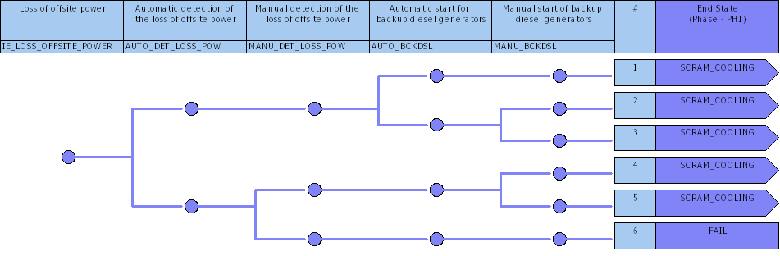
\includegraphics[height=0.25\textheight]{fig0c/Event/B1_LOSS_OFFSITE_POWER}
	\mycaption[Event tree for the loss of offsite power]{Event tree for the loss of offsite power.}
	\label{fig:event_power}
\end{figure}

\begin{figure}[H]
	\centering
	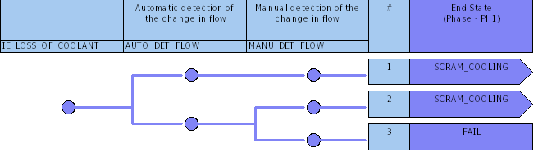
\includegraphics[height=0.2\textheight]{fig0c/Event/LOSS_OF_COOLANT}
	\mycaption[Event tree for the loss of coolant]{Event tree for the loss of coolant.}
	\label{fig:event_coolant}
\end{figure}

\begin{figure}[H]
	\centering
	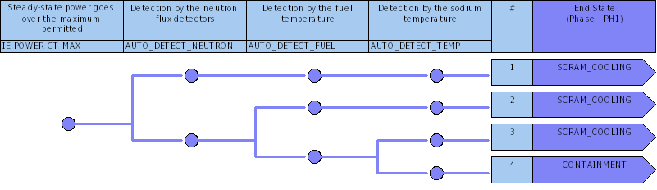
\includegraphics[height=0.2\textheight]{fig0c/Event/POWER_EXCURSION}
	\mycaption[Event tree for the power excursion]{Event tree for power excursion.}
	\label{fig:event_powexc}
\end{figure}

\begin{figure}[H]
	\centering
	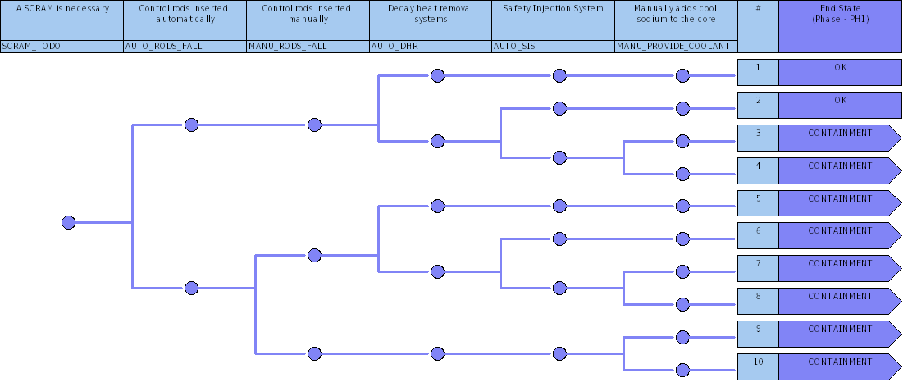
\includegraphics[height=0.3\textheight]{fig0c/Event/SCRAM_COOLING}
	\mycaption[Event tree for the SCRAM and cooling]{Event tree for the SCRAM and cooling.}
	\label{fig:event_scram}
\end{figure}

\begin{figure}[H]
	\centering
	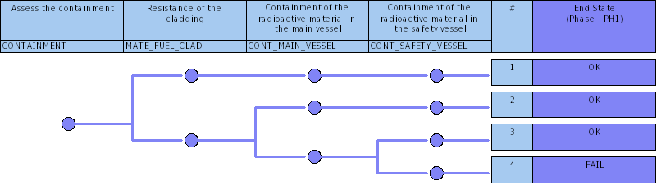
\includegraphics[height=0.2\textheight]{fig0c/Event/CONTAINMENT}
	\mycaption[Event tree for the containment]{Event tree for the containment.}
	\label{fig:event_cont}
\end{figure}

\begin{figure}[H]
	\centering
	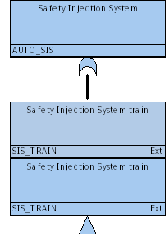
\includegraphics[height=0.25\textheight]{fig0c/Fault/AUTO_SIS}
	\mycaption[Fault tree for the safety injection system]{Fault tree for the safety injection system.}
	\label{fig:fault_sis}
\end{figure}

\begin{figure}[H]
	\centering
	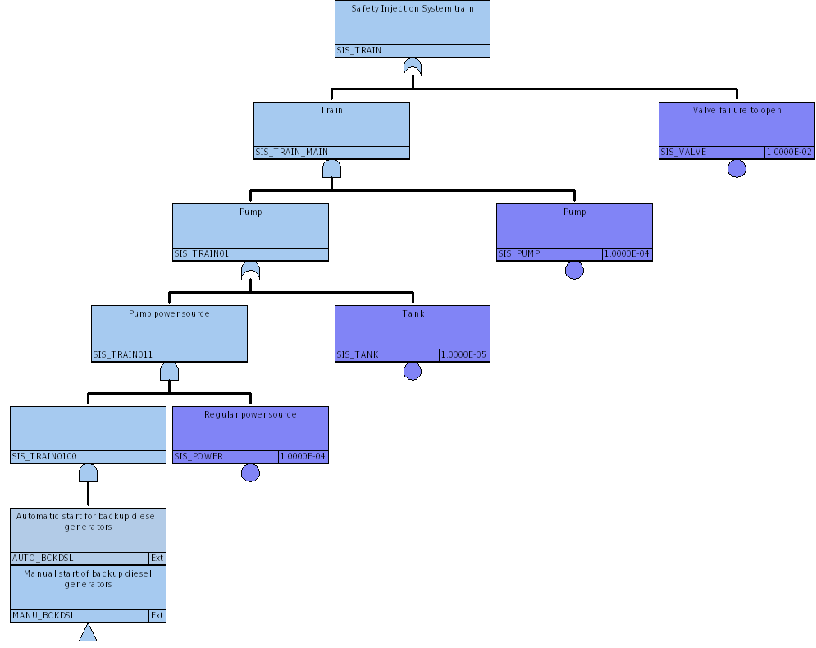
\includegraphics[height=0.5\textheight]{fig0c/Fault/SIS_TRAIN}
	\mycaption[Detailed fault tree for the safety injection system]{Detailed fault tree for the safety injection system.}
	\label{fig:fault_sis_d}
\end{figure}

\begin{figure}[H]
	\centering
	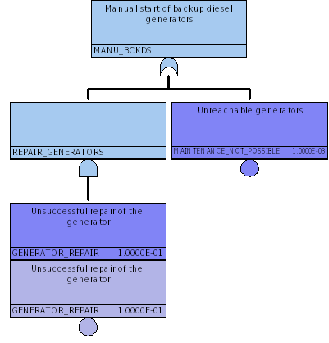
\includegraphics[height=0.4\textheight]{fig0c/Fault/MANU_BCKDSL}
	\mycaption[Fault tree for the manual use of the backup generator]{Fault tree for the manual use of the backup generator.}
	\label{fig:fault_bckgen}
\end{figure}

\
